\chapter{Experimentación}

\graphicspath{ {./graphs/} }

En este capítulo explicaremos todo el proceso de experimentación, desde la recogida de datos hasta la obtención de resultados como se ilustraba en el diagrama \ref{fig:full_pipeline}.



\section{Entorno}

Para poder llevar a cabo unos resultados validos seria necesario tener una planta solar capaz de producir energía y la monitorización de esta. En este caso, dispondriamos de la potencia actual generada, la cual es la entrada a los algoritmos de predicción. 

Dado que no es así, simularemos este comportamiento con un proceso manual de recogida y procesado de datos compuesto por una planta simulada con actuación sobre un historico.
La temperatura y radiación sera recopilada por un RESTful API, almacenada en una base de datos, extraida y formateada para ser introducida en el modelo de planta fotovoltaica de Matlab.
Tras ejecutar la simulación, los valores de potencia resultantes seran pasados a los distintos modelos para obtener las predicciones.
Una vez obtenidas las predicciones, seran contrastadas con los valores reales obteniendo asi graficas que prueben la certeza de estas.

A continuación se explican cada uno de los componentes del entorno.

\begin{itemize}
    \item Preprocesado
    \begin{itemize}
        \item RESTful API de pronostico climatologico dark sky
        \item Servidor
        \item Parser
    \end{itemize}
    \item Planta simulada
    \begin{itemize}
        \item Base de datos
        \item Modelo de planta solar
    \end{itemize}
    \item Algoritmos de predicción
\end{itemize}


\subsection{RESTful API} 
\label{sub:API}

El primer paso para la puesta en marcha del modelo de planta solar es recoger los valores de radiación y temperatura.

Para la recogida de datos barajamos estas opciones:
\begin{enumerate}
    \item Estación meteorologia de AEMET con valores reales de su base de datos
    \item API publica
\end{enumerate}


\subsubsection{Estación meteorológica de AEMET}
\label{ssub:estación_meteorológica_de_aemet}

Fue nuestra primera opción por ser una base de datos solida a la que tenemos acceso. Tiene puntos fuertes como proximidad, soporte técnico y fiabilidad.

En la estación meteorológica de Barajas

% \input{code/AEMET_db1.txt}

Unidades y valores especiales:

Horas UTC (Tiempo Universal Coordinado)


La insolación hace referencia la radiación solar \textbf{porcentual} y solo esta disponible en Barajas.
La temperatura en cambio solo esta disponible en Cuidad Universitaria y El Retiro.

Queda excluida la base de datos de AEMET.

API publica

Descartada la opción de estación meteorologica, nos inclinamos por una API RESTful publica y gratuita que proporciónase los valores necesarios: Temperatura e Irradiación ademas de Velocidad del viento y Dirección.

Las opciones fueron:
- Madrid AEMET opendata
- El tiempo
- solarelectricityhandbook.com/solar-irradiance.html
- National Renewable Energy Laboratory (NREL)
- dark sky weather

Tras optar por revisar otras fuentes, se observo que no es tan común disponer de un servicio que provisione la irraciación solar a nivel horário. El NREL dispone un API con la irradiación a nivel mensual, pero no es suficiente.

Tras ver que ninguno de estos trae valores reales de irradiación (temperatura todos) y dado que el objetivo es ver como se comportan los modelos de predicción en un escenario real, se opto por combinar la oclusión (La cobertura del cielo/nubes) con una funcion normal de 5 valores. La cantidad de sol recibida al día dibuja casi la misma gráfica cada día a lo largo de todo el año (Desfasada y/o ampliada en función de la estación). Las nubes son el mayor agravante, por ello las tomaremos como el factor importante. 

Finalmente nos quedamos con dark sky weather que era capaz de proporcionar todo (Temperatura, Covertura del cielo, Velocidad del viento y Dirección del viento).

Los datos necesarios para acceder al API son la url y la API KEY.

Con estos datos ya es posible realizar llamadas en forma de peticiones http y obtener los resultados.

Las funciones usadas fueron:

- Get token
- Get weather

%#TODO
%\lstinputlisting{./code/Darksky_ForecastRequest.txt}

A la hora de consultar el tiempo y las predicciones incluimos varias opciones para obtener resultados mas concisos.

%#TODO
%\lstinputlisting{./code/Darksky_ResponseFormat.txt}

Por lo tanto, el formato de las respuestas seria:
%\lstinputlisting{./code/Darksky_ResponseSample.txt}


\subsection{DB} 
\label{sub:DB}

Se ha elegido MongoDB como base de datos por no necesitar preparación para la inserción como podría ser crear una tabla en cualquier SQL DB. Esta es una de las ventajas de los documentos. Además no es necesaría ningun tipo de estructura relacional en los datos.


\subsection{Server} 
\label{sub:server}

Habiendo elegido la fuente de datos, es necesario automatizar la recogida y su almacenado.

Para ello se opto por una aplicación creada con el framework nodejs y una base de datos mongo.

Nodejs porque es versatil y comodo para tratar javascript con el.

El servidor se encarga de realizar periodicamente las llamadas a la API de dark sky, anadir la fecha de la llamada (por claridad, ya que los las fechas estan representadas segun la base de tiempo POSIX*), quitar las predicciones horarias excepto del principio del dia e insertar las respuestas en la base de datos.

La arquitectura esta montada en un Ubuntu Desktop 16.04 y dockerizada que permiten desacoplar el software del hardware y proporcionan resiliencia*

Finalmente el servidor esta emplazado fisicamente en [la facultad de informatica(?)] 



\subsection{Extractor de datos} 
\label{sub:extractor_de_datos}

Una vez tenemos la base de datos con contenido suficiente en continuo crecimiento, ya se puede proceder a extraer los datos de la base de datos y pasarselos al modelo de planta fotovoltaica de simulink para que proporcione una potencia de salida.

Para ello, realizaremos una consulta a la base de datos y escribiremos los resultados en un archivo de texto que reconozca Matlab y facilite su manipulación.

A lo largo del desarrollo se han implementado 2 tipos: Como txt donde cada linea tiene datos separados por tabulaciones y como json.

Dado que la base de datos no contiene el 100\% de los datos (Se escapan alrededor de 2-4 entradas por mes) se rellenan esos datos con el valor mas próximo a fin suprimir posibles outliers.

%#TODO
[Codigo explicado]

Con esto tenemos los ficheros preparados.
%#TODO
[json y txt samples]



\subsection{Matlab}
\label{sub:Matlab} 

Para la implementación de los modelos se ha optado por usar Matlab ya que a diferencia de C++ u otros lenguajes, tiene un toolbox de diseño de redes neuronales muy completo y practico.

La primera función de Matlab será extraer los valores de los json de la fase anterior y crear una señal para el modelo de Simulink. Una vez hecho esto se podrá comenzar la simulación y obtener los resultados. Hecho esto se discretiza la señal de salida para ajustarla al formato de horas y días para finalmente pasarselo a los modelos.


\subsection{Simulink}
\label{sub:Simulink}

El siguiente modelo simula una planta fotovoltaica de 100kW. 

\begin{figure}[h]
    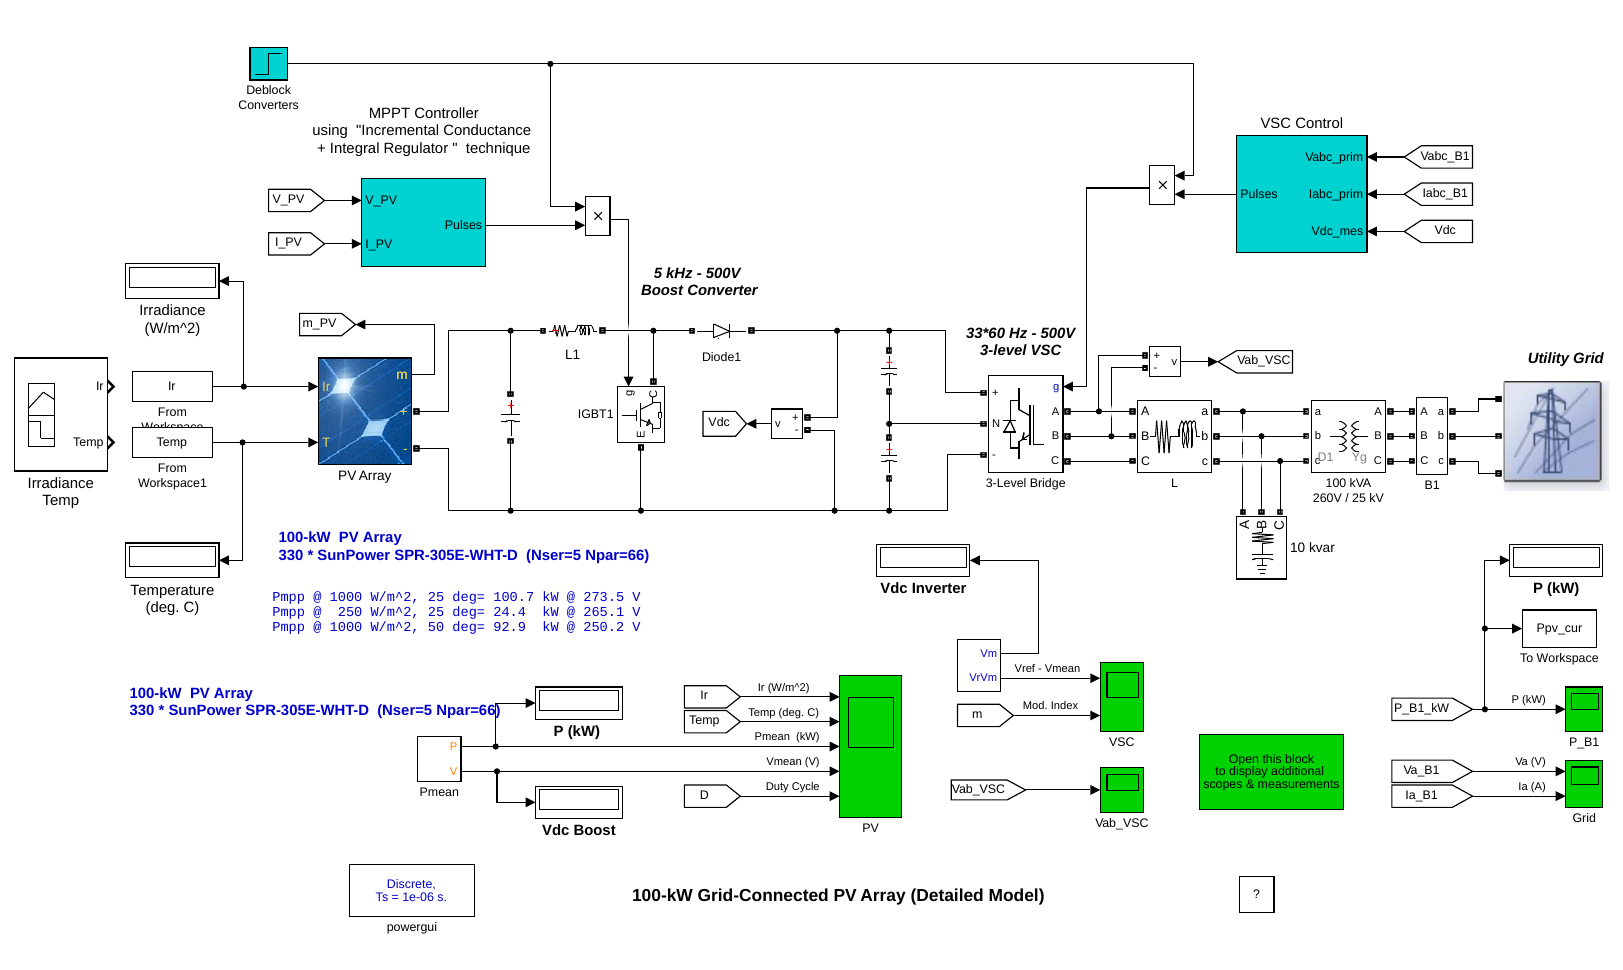
\includegraphics[width=\textwidth]{Ppv_diagram.png}
    \caption{Diagrama de la planta fotovoltaica de 100kW conectada a una red}
    \label{fig:Ppv_diagram}
\end{figure}


El modelo simula una planta fotovoltaica con las siguientes características:
\begin{itemize}
    \item 100kW a 1000$W/m^2$
    \item Conectada a una red de 25kV de tres fases
    \item Conexión DC-DC con amplificador de tensión
    \item 1980-Hz con VSC de 3-niveles y 3-fases
    \item Condensador de 10kvar para el filtrado
\end{itemize}

Para llevar a cabo la simulación es necesario introducir las variables mas relevantes para el panel fotovoltaico: Radiación y Temperatura. Tiene como resultado la potencia instantanea en watios. El modelo evalua las entradas 1000 veces por segundo dando como resultado una detallada grafica de potencia producida.

La importación y exportación de los valores se ha realizado desde el workspace, donde se pre y post procesan las señales resultantes: Las entradas (Radiación y Temperatura) se formatean de acuerdo a las entradas del modelo y las salidas (La potencia) se discretiza a valor por hora, ya que se evalua la potencia a un ratio de 1000 veces por 1 segundo de simulación.

La quicena de potencia que usaremos es la descrita entre el 1 y el 16 de abril. Se puede observar en la gráfica \ref{fig:Ppv_output} donde el eje x son los dias y el y la potencia generada en watios.

El resultado de la simulación puede observarse en la siguiente figura:

\begin{figure}[h]
    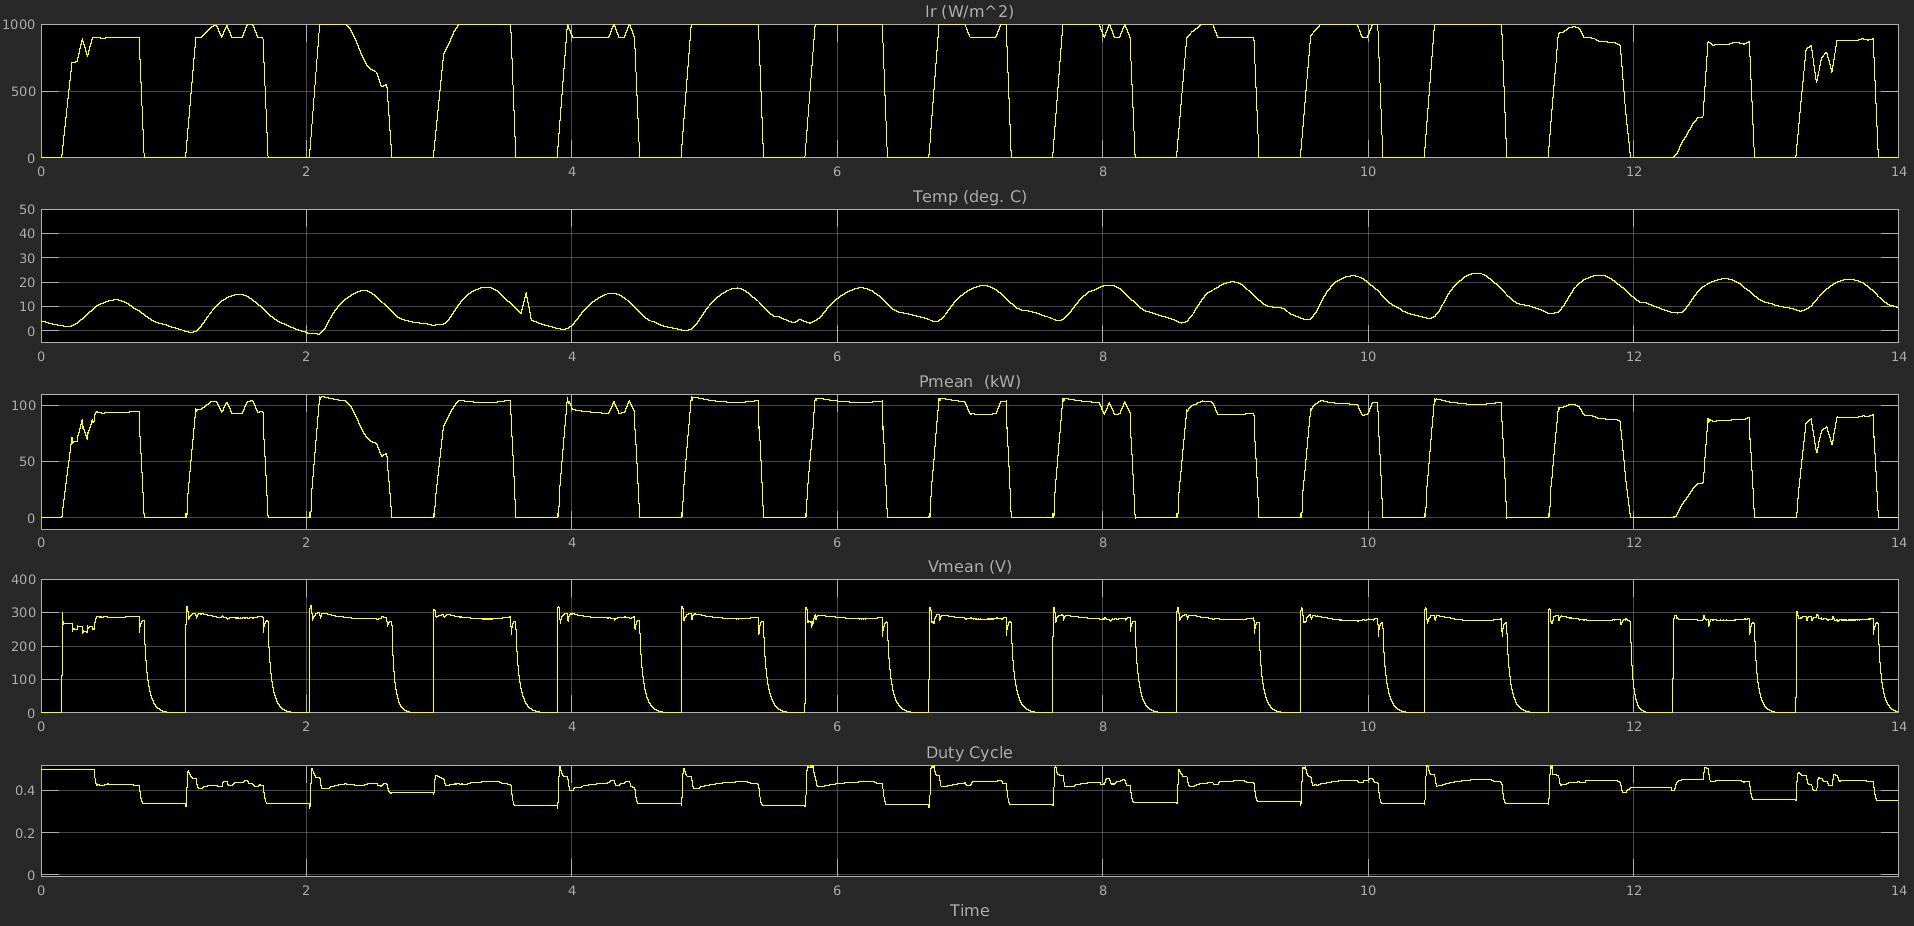
\includegraphics[width=\textwidth]{Model_cur_outputs_010417.jpg}
    \caption{Salida de la planta fotovoltaica}
    \label{fig:Ppv_output}
\end{figure}


\subsection{Modelos}

A fin de desacoplar lo maximo posible la prediccion de otras etapas (Como importación del fichero, simulación o procesado de la señal de salida), los modelos leerán la variable del workspace $E_cur$ cuyo formato se que sea filas = días, columnas = horas

En función del algoritmo y la cantidad de operaciones a nivel horário se optará por trasponer y hacer los accesos aprovechando el acceso de índice único de Matlab a fin de poder tratar de manera más cómoda.

Todos los modelos estan preparados para realizar una única predicción con las constantes definidas (Sin etapa de ajuste como podría ser realizar una predicción con cada constante y elegir la menor dispersión) y mostrar el resultado final con una comparación entre valores reales - predichos y el error.

\subsubsection{N4SID}
\label{ssub:n4sid}

Consideraremos también un N4SID (Algorítmo numérico para identificación de sistemas de espacios de subespacios de estados) y su implementación de Matlab. Con la función $m = n4sid(data,order,'Property1',Value1,...,'PropertyN',ValueN)$, siendo m el modelo resultante [idss], data la entrada y salida [idss], order el valor de nx que en este caso dejaremos en 'best' el cual escogerá el mejor entre 1 y 10, y finalmente pares propiedad-valor, que unicamente usaremos N4Horizon, que define el horizonte de predicción y será 24h.

Para este modelo de predicción tomaremos los valores de salida del modelo de simulink $pe_asm_generator_2$ separandolos en 75\% para entrenamiento y 25\% para validación. 

Lo más importante para que funcione adecuadamente, no solo el modelo sino también un molino real, es que la velocidad se encuentre entre 3 y 23m/s. De otro modo la salida será 0.

Entrenamos realizando un bucle entre 8 y 168 que representan los valores del pasado tomados para el entrenamiento. Entre 1/3 de día y 7 días. Guardando en cada iteración el valor de ajuste para finalmente crear el modelo con los valores finales.



\subsubsection{ARMA/ARIMA}
\label{ssub:arma_arima}

Para realizar la predicción con alguno de estos modelos primero habría que estudiar si la serie a tratar es estacionaria (Se realiza solo con la de entrenamiento). Si es estacionaria, se puede omitir la Integración (ARMA) si no, ARIMA.

Hay dos tipos de estacionariedad, en media y en varianza, 

%#TODO

